
\section{La ricerca}
	In base al numero di pagine la funzionalità di ricerca diventa fondamentale in un sito internet. Nel caso di cinisio.com dalle analisi fatte con strumenti online le pagine risultato essere \textbf{quasi 300} (figura \ref{fig:NumeroDiPagine}).
	
	
	\begin{figure} [h]
		\centering
		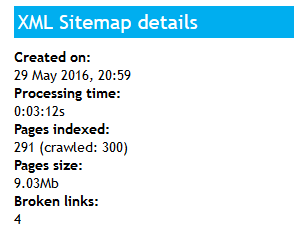
\includegraphics[width=0.5\textwidth]{images/NumeroDiPagine}
		\caption{Numero di pagine dopo l'analisi con il tool \textit{XML Sitemap}}
		\label{fig:NumeroDiPagine}
	\end{figure}
	
	In tal caso è necessario dotare il sito di una funzionalità di ricerca ma questa non c'è. Infatti nella homepage non troviamo nessuna casella di ricerca (search box) e solo dopo aver controllato attentamente si trova il link ad una presunta ricerca nella didascalia dell'immagine in primo piano (figura \ref{fig:Homepage-Ricerca}).
	
	\begin{figure} [h]
		\centering
		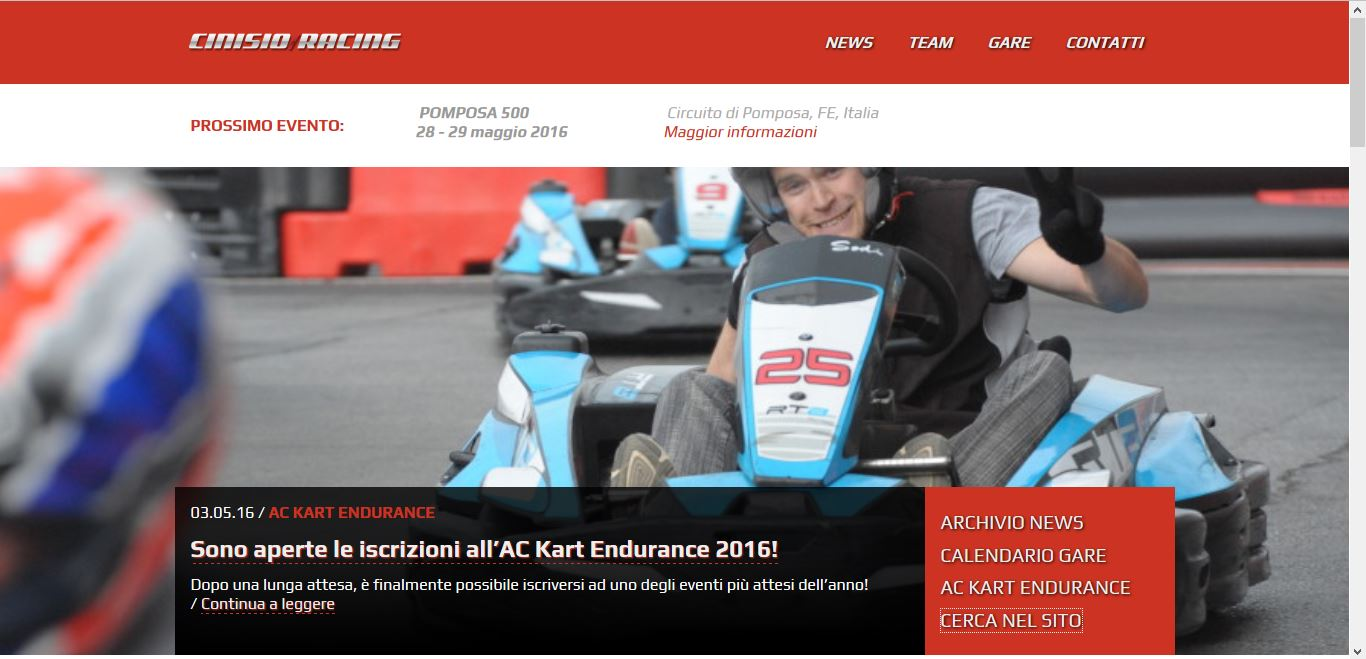
\includegraphics[width=\textwidth]{images/SearchOption_WhereItIs}
		\caption{Il link per la ricerca nel sito}
		\label{fig:Homepage-Ricerca}
	\end{figure}
	
	Il link però porta alla pagina con il messaggio in figura \ref{fig:RicercaNonDisponibile} e subito dopo aver descritto che la funzionalità non è implementata nel sito incoraggia l'utente ad utilizzare un search box a lato nella pagina. 
	
	\begin{figure} [h]
		\centering
		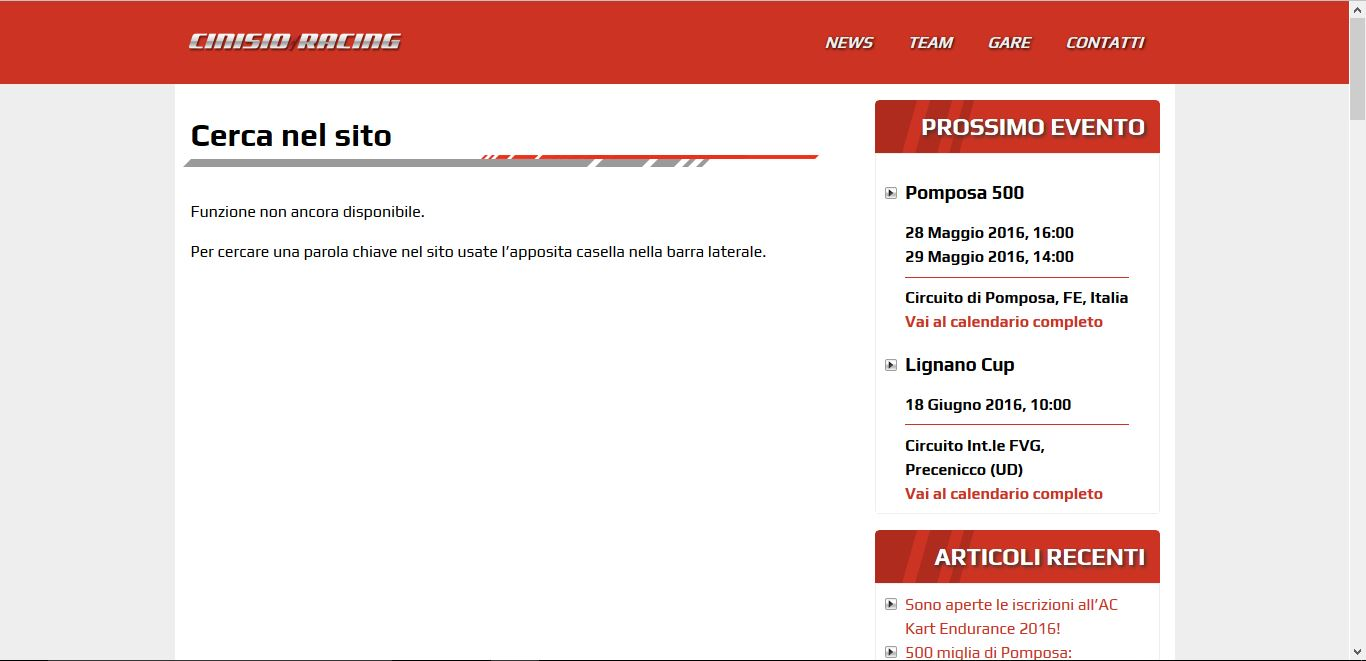
\includegraphics[width=\textwidth]{images/PoorSearchBox}
		\caption{L'avviso contraddittorio il quale dice che la funzionalità di ricerca nel sito non è presente ma è disponibile a lato}
		\label{fig:RicercaNonDisponibile}
	\end{figure}
	
	L'utente così paziente da leggere anche la seconda riga dell'avviso si accorgerà quindi che effettivamente esiste un search box situato a lato dopo uno scroll e solo in alcune pagine del sito (figura \ref{fig:RicercaSearchBox}). La posizione nascosta sembra intenzionale per scoraggiarne l'uso -- oltre a scoraggiare il proseguimento della navigazione nel sito -- ma alcune prove effettuate con la search box trovata rivelano che la funzionalità di ricerca c'è e funziona abbastanza bene. Dalla figura \ref{fig:RicercaRisultati} possiamo vedere come una semplice ricerca con le keyword \textit{Kart} e \textit{endurance} hanno prodotto una lista di risultati coerente con le attese.
	
	\begin{figure} [h]
		\centering
		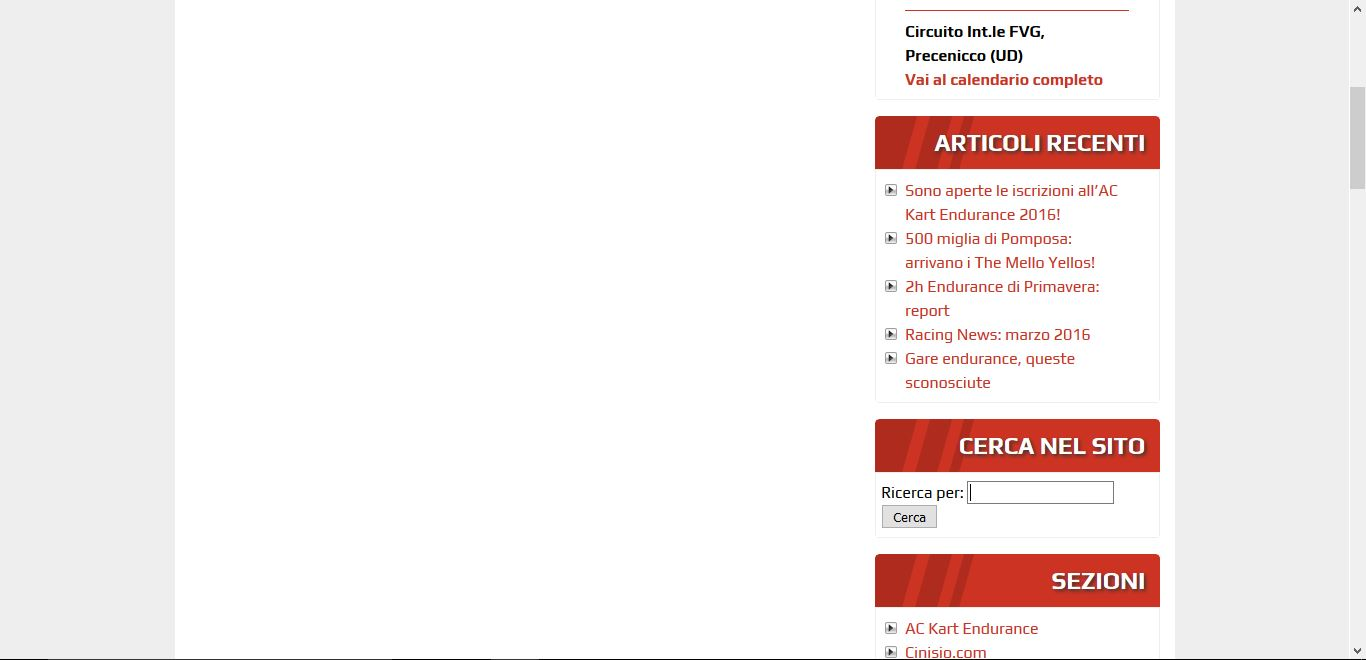
\includegraphics[width=\textwidth]{images/FinallyTheSearchBox}
		\caption{La posizione del search box in alcune pagine del sito}
		\label{fig:RicercaSearchBox}
	\end{figure}
	
	\begin{figure} [h]
		\centering
		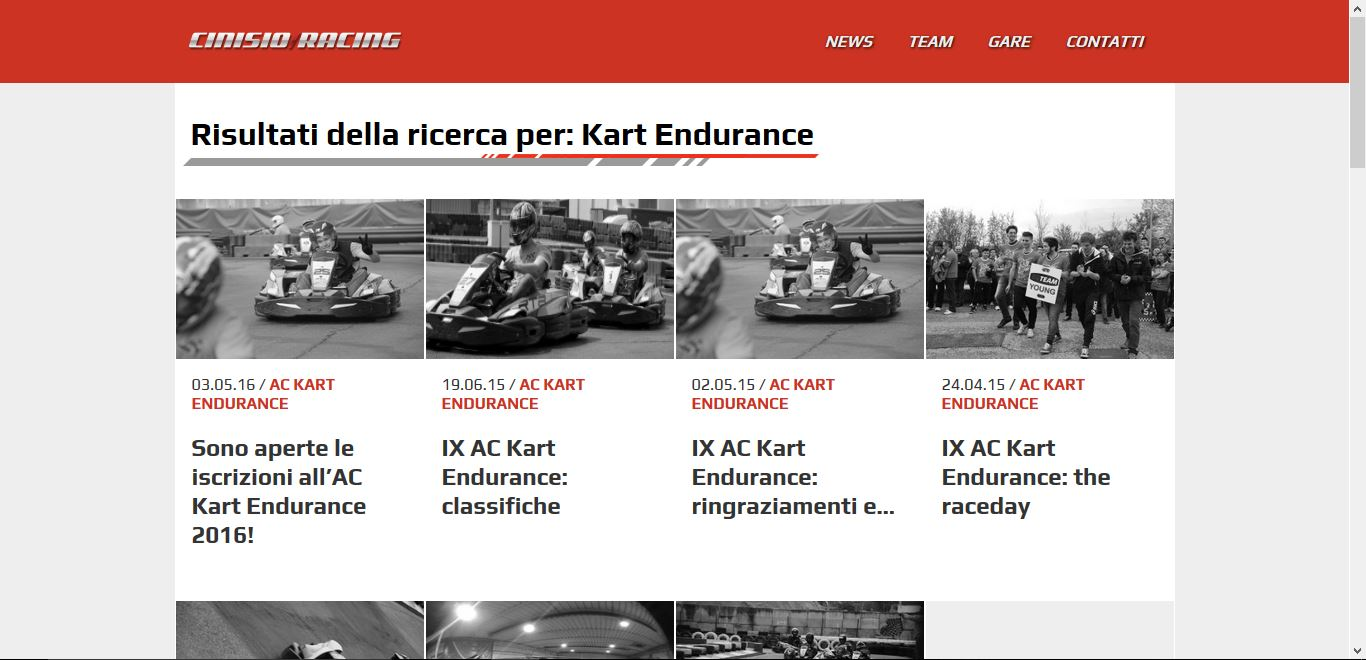
\includegraphics[width=\textwidth]{images/SearchResult}
		\caption{I risultati della ricerca delle keyword \textit{Kart Endurance}}
		\label{fig:RicercaRisultati}
	\end{figure}
	
	Per un tecnico della materia è evidente che nel sito sono presenti due ricerche differenti: una molto più raffinata ma non implementata e una più imprecisa ma già implementata. Il problema è che il passaggio da una all'altra deve essere fatto senza lasciare l'utente disorientato con un messaggio d'avviso contraddittorio. 
	La search box deve essere messa bene in vista, anche nella homepage, non importa se non porta a risultati precisi, all'utente deve essere data l'opportunità di ricercare all'interno di un sito composto da quasi 300 pagine.